\chapter{针对新型加速器性能模拟器}

我们提出的粗粒度稀疏的神经网络加速器Cambricon-S能够充分利用粗粒度稀疏神经网络的神经元/索引共享和负载均衡等特性,同时利用动态神经元稀疏和局部量化进一步减少计算量和访存量,从而提升加速器性能,减少能耗。

我们采用模拟的方法对新型加速器进行性能分析。传统的周期精确模拟器由于性能低,速度慢,无法满足我们实际的需求。因此,我们为Cambricon-S设计了一个专用性能模拟器,它能够在误差允许范围内快速进行性能模拟。

优化的性能模拟器基于事件驱动进行设计,它能够隐藏加速器中复杂的设计细节,专注于影响加速器性能的因素,从而快速,准确地预测神经网络在新型加速器上的执行时间。

\section{背景}
计算机模拟是指利用计算机软件开发的模拟器对真实世界过程或者系统进行模拟的行为,进而完成故障分析、测试 VLSI逻辑设计等复杂的任务,从而为研究人员提供设计指导。计算机系统模拟器是指以在一台计算机上模拟另一台指令不兼容或者体系不同的计算机。如今,计算机系统模拟器已经成为了计算机系统结构领域研究中不可或缺的工具。研究人员通过使用模拟器能够用较低的成本和开销,高效地完成对软硬件的配置和观察,进而为硬软件的设计和优化提供指导。随着计算机行业的迅猛发展,计算机功能变得越来越强大的同时,计算机系统也变得越来越复杂,模拟计算机系统的开销也越来越大,因此如何提升模拟器的性能成为一个亟待解决的问题。研究者一般从准确性,事件开销,内存开销,易用性和可扩展性这几个方面考虑模拟器的性能。

研究者一般采用周期精确模拟器进行硬件的性能模拟。周期精确模拟器需要模拟硬件的每一个模块在每一个时钟周期执行操作的各个细节,包括状态机跳转,寄存器更改,流水级操作等,以保持模拟器与硬件之间的一致性。这种精确模拟会导致巨大的资源,能源和时间开销,进而导致周期精确的模拟器无法满足实际的需求。

周期精确的模拟器按照实现方式可以分为两类,一类是时间触发的模拟器,一类是事件触发的模拟器。其中时间触发模拟器以cycle为单位进行模拟,每一个cycle会触发一次模拟操作;事件触发模拟器以事件为单位进行模拟,事件通常为用户自定义事件,每一个事件会触发一次模拟操作。如图~\ref{fig:event}所示,一个浮点乘法单元需要产生一个浮点乘法操作,该浮点乘法需要三个周期完成。当我们使用时间触发的模拟器时,总共需要模拟四个周期的浮点乘法操作,尽管第二个和第三个周期内不需要进行任何模拟操作;当我们使用事件触发的模拟器时,只需要模拟两个周期的操作就能完成。由于神经网络加速器涉及到大规模数据的传输和运算,基于事件触发的模拟器更有性能上的优势。

\begin{figure}[h]
\centering
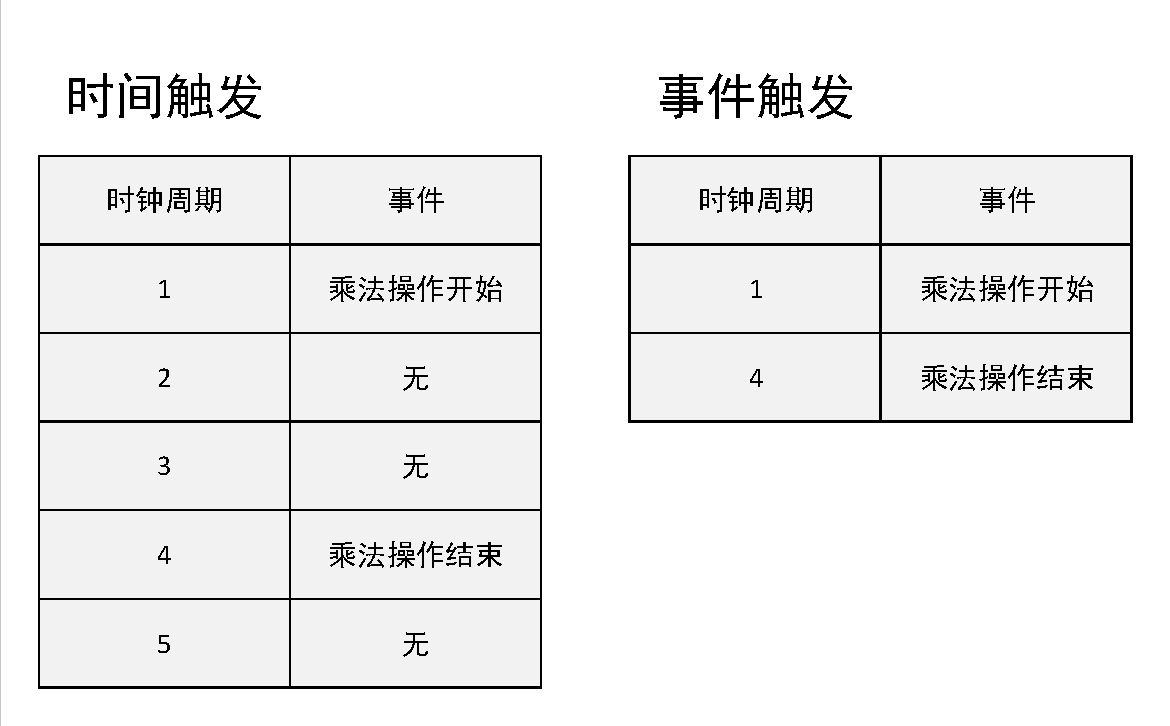
\includegraphics[width=1.0\columnwidth]{event.pdf}
\caption{时间触发模拟器和事件触发模拟器}
\label{fig:event}
\end{figure}

\section{加速器专用性能模拟器}

我们采用基于事件触发的模拟器对Cambricon-S进行性能模拟。在设计性能模拟器的过程中,我们采用了如下的策略优化模拟器,在误差允许范围内加快模拟速度,提高模拟器的性能:第一,我们对加速器进行高层次抽象,隐藏加速器中复杂的细节,只关注影响性能的最主要因素,从而简化性能模拟器的设计,加快性能模拟器的模拟速度。第二,我们精简了模拟器中的事件,提取出最重要的事件构建神经网络的执行过程,同时我们使用建模的方法计算事件的执行时间,提高模拟器的准确性。第三,我们根据loop tiling将神经网络的执行过程分为多个子运算,然后我们以子运算为单位进行性能模拟,最终通过累加各个子运算的执行事件获得神经网络在加速器上的运行时间。


\subsection{加速器的高层次抽象}

\begin{figure}[h]
\centering
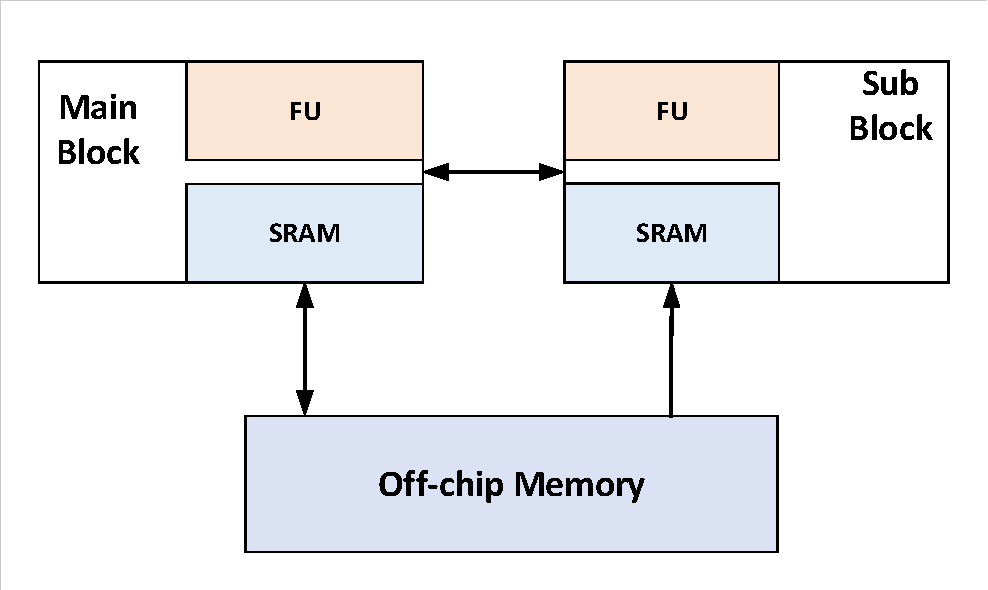
\includegraphics[width=1.0\columnwidth]{simulator.pdf}
\caption{加速器的抽象结构}
\label{fig:simulator}
\end{figure}

为了简化性能模拟器的设计,加快性能模拟器的模拟速度,我们首先需要对新型加速器进行高层次的抽象,隐藏新型加速器的细节,提取出影响神经网络执行速度的关键因素。由于新型加速器中的大部分模块内部采取流水(pipeline)的方式执行,而且部分模块之间也完成了流水操作,因此我们可以将这些流水的模块整合为一个大模块,从而隐藏新型加速器的设计细节。

如图~\ref{fig:simulator}所示,新型加速器的抽象结构由三部分构成,分别是Main Block, Sub Block和Off-chip Memory。下面我们将对这三个部分进行详细介绍。

\subsubsection{Main Block}
Main Block主要作为数据通路同时,完成一部分向量运算和标量运算。Main Block由片上缓存SRAM,运算单元FU(functional unit)组成。
Main Block中的SRAM对应了新型加速器中的四个片上缓存,分别是NBin,NIBin,NBout和SIB。Main Block中的FU主要用来完成向量运算,标量运算和非线性运算。其中向量运算包括逐元素相加,逐元素相乘等运算;标量运算包括标量四则运算;非线性运算主要包括指数,双曲函数等超越函数,用来支持激活函数运算。Main Block中主要完成Pooling层,BN层,ROI Pooling层和激活层的运算。

值得注意的是,Main Block的内部集成了新型加速器中的稀疏处理的模块,如NSM,SSM,Encoder等,由于选数逻辑与运算逻辑之间为流水的结构,只要我们能够准确模拟运算模块的性能,是否模拟这些模块对最终的结果没有影响,因此我们可以隐藏这些模块的细节,专注于加速器中运算模块的模拟,因此我们将这部分稀疏处理模块隐藏。

\subsubsection{Sub Block}
Sub Block主要是核心运算模块,主要完成神经网络算法中的矩阵向量运算。Sub Block由片上缓存运算SRAM和运算单元FU构成。Sub Block中的SRAM对应新型加速器中的SB,FU则对应了PEFU。神经网络中的卷积层,全连接层和LSTM层的大部分运算都在Sub Block的FU中完成。

\subsubsection{Off-chip}
Off-chip Memoy存储了神经网络的参数,包括神经网络的拓扑结构,输入,权值,部分和,输出等。由于加速器的片上缓存有限,加速器无法一次性将神经网络的所有参数存储到片上缓存,因此Off-chip Memory与片上缓存之间需要由非常频繁的数据交换。

\subsubsection{数据通路}
Main Block与Sub Block之间存在数据双向的数据通路,从Main Block到Sub Block方向的通路用来传输输入神经元,从Sub Block到Main Block方向的通路用于传输输出神经元部分和。

Main Block与Off-chip Memory之间也存在双向数据通路,其中从Off-chip Memory到Main Block方向的通路用来加载输入神经元,输入神经元索引,输出神经元部分和和权值索引,从Main Block到Off-chip Memory方向的通路用来存储输出神经元部分和。

Sub Block与Off-chip Memory之间仅仅存在单向的数据通路,从Off-chip Memory到Sub Bloock方向的通路用来加载权值。


\subsection{事件分类}
设计基于事件触发的模拟器,我们首先需要根据加速器的特性和数据流定义在加速器在运行神经网络过程涉及到的事件。事件有一个四维的描述符,分别是类型,数据,时刻和时间,其中类型用来描述事件需要完成的操作,包括控制(如分支跳转),访存(如Load/Store片外DDR或者Read/Write片上缓存),运算(如矩阵,向量,标量,逻辑运算等);数据描述事件涉及到的数据,包括数据地址,数据大小,数据类型等信息;时刻描述了事件出触发的时间点;时间描述了事件的执行时间,执行时间可以通过性能分析(Profiling)或者建模(Modeling)的方式完成。

我们在新型加速器的性能模拟器中定义了四个事件,分别是数据加载事件,运算事件,数据存储事件和同步事件,我们将它们依次简写为Load事件,Compute事件,Store事件和Synchronize事件。

\subsubsection{Load事件}
Load事件涉及到将数据从Off-chip Memory加载到Main Block的SRAM和Sub Block的SRAM中;对应到新型加速器中,就是将输入神经元,输入神经元索引,输出部分和,权值和权值索引分别从片外加载到NBin,NIBin,NBout,SB和SIB中。

\subsubsection{Compute事件}
Compute事件涉及到Main Block中的FU和Sub Block中的FU完成神经网络的核心运算,神经网络运算包括矩阵运算,向量运算和标量运算。

其中矩阵运算主要包括矩阵向量运算,这部分是神经网络的核心运算,卷积层,全连接层,LSTM层中大部分运算都是矩阵向量运算。

向量运算包括向量内积,向量逐元素相乘,向量逐元素相乘,神经网络中的池化层,BN层,LSTM层,LRN层等都是涉及到向量运算。

标量运算主要包括标量的四则运算,Faster-RCNN中的ROI pooling层会涉及到这部分的运算。

因此,Compute事件还能进一步划分矩阵运算事件(Matrix Compute),向量运算事件(Vector Compute)和标量运算事件(Scalar Compute)。

\subsubsection{Store事件}
Store事件涉及到将Main Block SRAM中的数据存储到Off-chip Memory;对应到新型加速器中,就是将输出部分和从NBout存储回Off-chip Memory。值得注意的是NBin,NIBin,SB和SIB这四个缓存不会涉及到Store事件。

\subsubsection{Synchronize事件}
Synchronize事件是一个同步事件。当出现Synchronize事件时,必须要保证Synchronize事件之前其他所有事件完成之后才能执行Synchronize事件之后的其他事件,也就是说Synchronize事件相当与一个同步信号,用来同步Synchronize事件之前的其他事件。

\subsection{事件执行时间}
我们采用建模的方式预测各个事件的执行时间,下面我们将详细介绍Load事件,Compute事件和Store事件的建模方法。值得注意的是,由于Synchronize事件是一个阻塞事件,用于同步之前所有的事件,因此不需要对其进行建模。

\subsubsection{对Load事件进行建模}
Load事件的执行时间跟数据量和Off-Chip Memory带宽有关,具体可以用如下方式进行计算
\begin{equation}
t_{Load} = t_{start} + Data_{Load} / Bandwidth_{Load}
\end{equation}
其中$t_{Load}$是Load事件执行时间,$t_{start}$是Off-chip Memory的启动时间,$Data_{Load}$是Load事件涉及到的数据量(包括所有输入神经元,输入神经元索引,输出部分和,权值和权值索引),$Bandwidth_{Load}$是Off-Chip Memory的Load带宽。

\subsubsection{对Compute事件进行建模}
Compute事件的执行时间与运算量和运算单元数量有关,具体可以用如下方式进行计算
\begin{equation}
t_{Compute} = Data_{Compute} / (FU * u\%)
\end{equation}
其中$t_{Compute}$是Compute事件执行时间,$Data_{Compute}$是Compute事件涉及的运算量,$FU$是运算单元的数量,$u\%$是运算单元的利用率。

神经网络的 神经元稀疏度,权值稀疏度,网络拓扑结构(如卷积层的规模,全连接层的规模),数据阻塞等因素都会影响运算单元的利用率,因此运算单元的利用率是一个实时的值。我们采用建模的方法计算运算单元的利用率进行预测,例如对于神经网络的卷积运算,我们会实测多组不同网络规模配置和稀疏度配置下运算单元利用率,然后根据这些数据对运算单元利用率进行建模,最终获得运算单元利用率与网络配置和稀疏度的定量关系。值得注意的是Matrix Copmute事件,Vector Compute事件和Scalar事件的执行时间都可以用上述公式进行计算。

\subsubsection{对Store事件进行建模}
Store事件的执行时间计算方法与Load时间类似,执行时间跟数据量和Off-Chip Memory带宽有关,具体可以用如下方式进行计算
\begin{equation}
t_{Store} = t_{start} + Data_{Store} / Bandwidth_{Store}
\end{equation}
其中$t_{Store}$是Store事件执行事件,$t_{start}$是Off-chip Memory的启动时间,$Data_{Store}$是事件涉及到的数据量(输出部分和),$Bandwidth_{Store}$是Off-Chip Memory的Store带宽。


\subsection{事件的依赖关系}
由于Cambricon-S中集成了多发射控制器~\ref{subsec:control},因此可以同时发射没有依赖关系的指令。在Cambricon-S中,没有依赖关系的指令包括三个方面,第一,IO指令与计算指令之间没有依赖关系;第二,Load和Store指令之间没有依赖关系;第三,如果计算指令涉及到涉及不同的计算单元和数据,那么这些计算指令之间也没有依赖关系。

对应的,性能模拟器也存在没有依赖关系的事件:第一,Load/Store事件与Compute事件之间没有依赖关系;第二,Load事件与Store事件之间没有依赖关系;第三,Matrix Compute事件,Vector Compute事件和Scalar事件之间没有依赖关系。没有依赖关系的事件可以同时执行,我们用Synchronize事件来同步没有依赖关系的事件。

\subsection{模拟过程}

\begin{figure}[h]
\centering
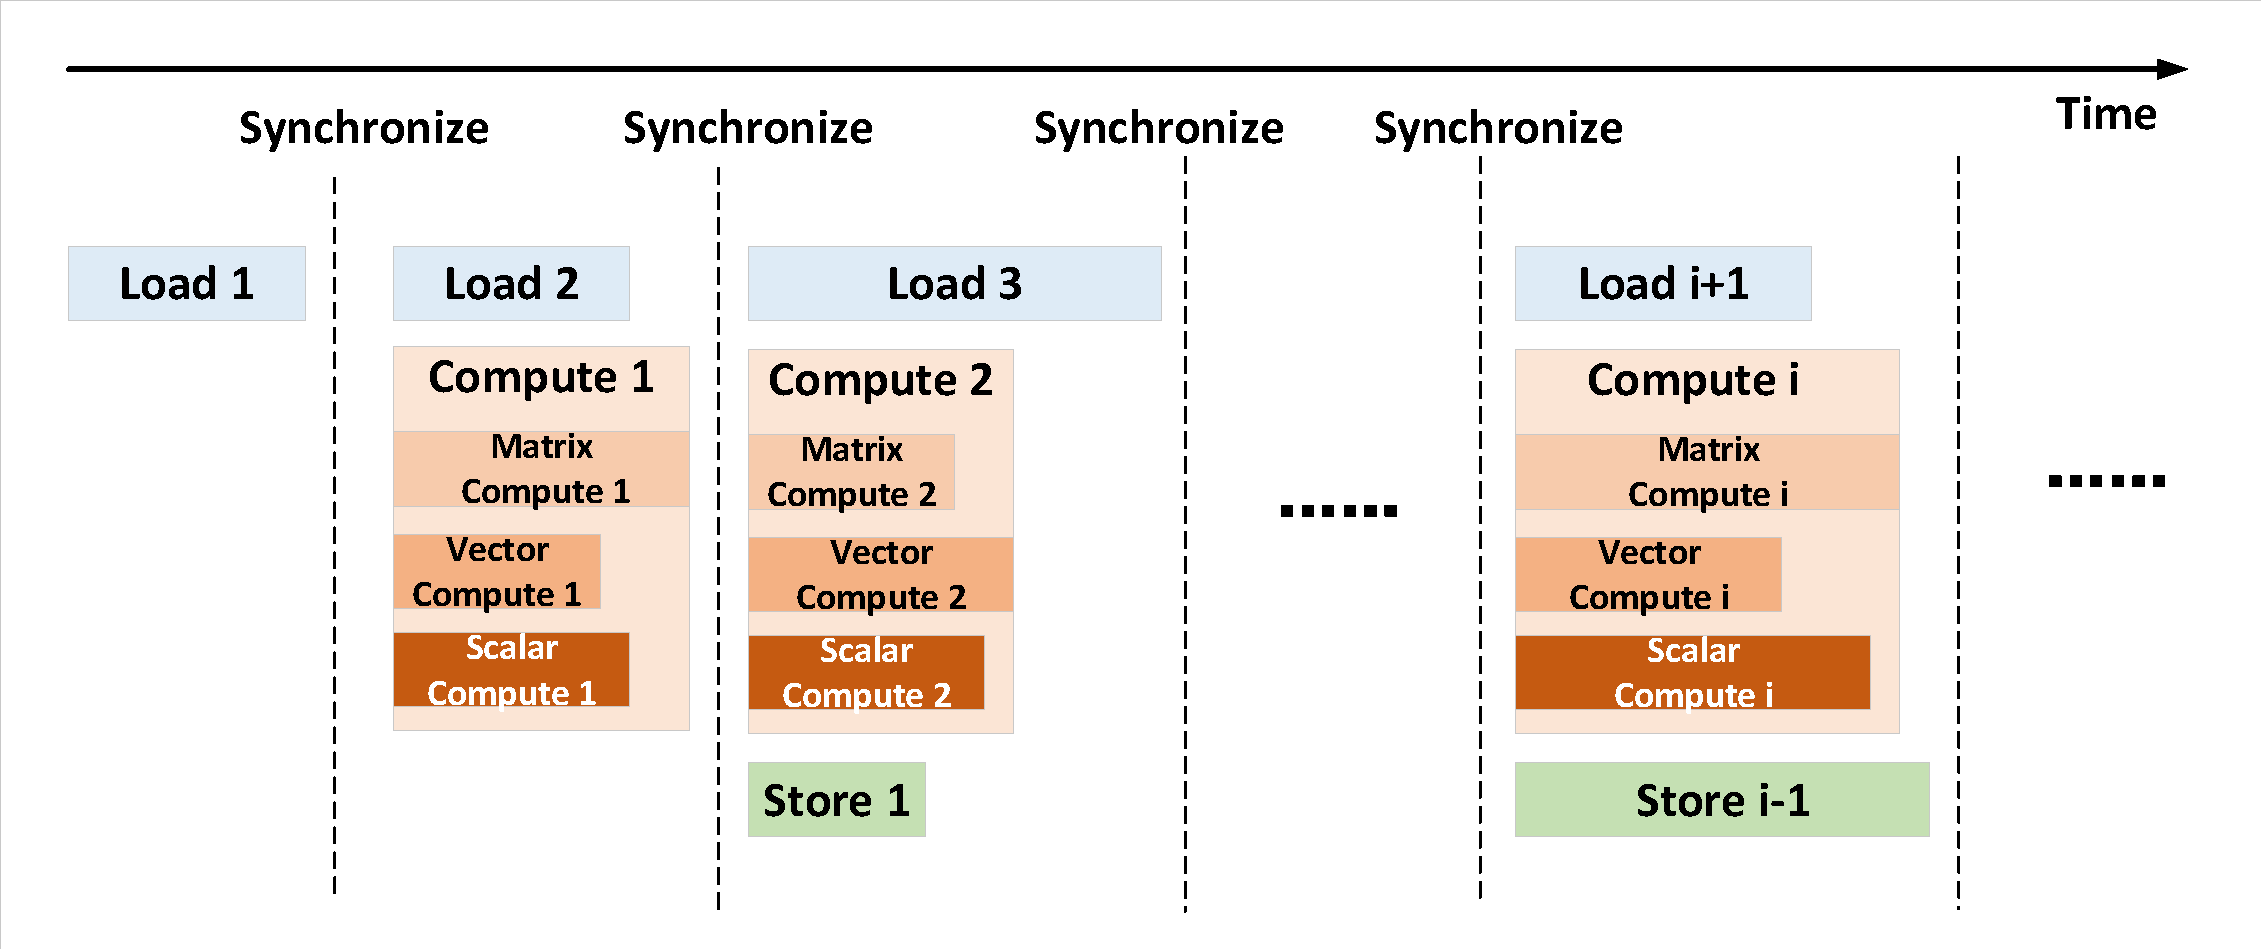
\includegraphics[width=1.0\columnwidth]{simulation.pdf}
\caption{性能模拟器模拟神经网络在加速器上的执行过程}
\label{fig:simulation}
\end{figure}

我们使用loop tiling的策略将神经网络运算分割成为多个子运算操作,使得每一个子运算对应的数据能够被完整加载到片上缓存中。假设神经网络某一层的运算被切分成为\emph{N}个子运算,同时\emph{N}个子运算对应\emph{N}个数据块。如图~\ref{fig:simulation}描绘了模拟器模拟神经网络在加速器上执行,同时统计运行时间的过程。神经网络的执行过程被分为\emph{N+2}个\emph{Step},两个\emph{Step}之间用\emph{Synchronize}事件进行分割,最终神经网络的执行时间是这\emph{N+2}个\emph{Step}的执行事件总和。

\emph{Step 1}:性能模拟器会触发\emph{Load 1}事件。\emph{Load 1}事件将第一个子运算对应的数据从Off-chip Memory加载到Main Block和Sub Block的SRAM中。此时由于片上缓存没有数据,Main Block和Sub Block的FU无法进行计算。然后我们使用\emph{Synchronize}事件进行同步。\emph{Step 1}的执行时间就是\emph{Load 1}事件执行时间。

\emph{Step 2}: 性能模拟器触发\emph{Load 2}事件和\emph{Compute 1}事件。其中\emph{Load 2}事件将第二个子运算对应的数据从Off-chip Memory加载到Main Block和Sub Block的SRAM中。此时由于片上缓存已经存储了第一个子运算对应的数据(经过\emph{Step 1}的\emph{Load 1}事件),所以模拟器会触发\emph{Compute 1}事件,Main Block和Sub Block的FU完成第一个子运算。值得注意的是,\emph{Compute 1}事件包括\emph{Matrix Compute 1}事件,\emph{Vector Compute 1}事件和\emph{Scalar Compute 1}事件这三个没有依赖关系的事件。最终\emph{Step 2}的执行时间取决于\emph{Load 1}, \emph{Matrix Compute 1}, \emph{Vector Compute 1}和\emph{Scalar Compute 1}这四个事件的执行时间的最大值。在图~\ref{fig:simulation}的示例中,\emph{Step 2}的执行事件取决于执行最慢的~\emph{Matrix Compute 1}事件。
为了表示方便,我们将\emph{Computen i}事件执行时间定义为\emph{Matrix Compute i}, \emph{Vector Compute i}和\emph{Scalar Compute i}这三个事件中执行时间的最大值。

\emph{Step 3}: 性能模拟器触发\emph{Load 3}事件,\emph{Compute 2}事件和\emph{Store 1}事件。其中\emph{Load 3}事件将第三个子运算对应的数据从Off-chip Memory加载到Main Block和Sub Block的SRAM中。\emph{Compute 2}事件开启Main Block和Sub Block的FU完成第二个子运算。 此时,由于Main Block的SRAM中存储了第一个子运算对应的结果(经过\emph{Step 2}的\emph{Compute 1}事件),模拟器触发\emph{Store 1}事件,将第一个子运算的运算结果存储到Off-Chip Memory。
最终\emph{Step 3}的执行时间是\emph{Load 3}, \emph{Compute 2}和\emph{Store 1}这三个事件执行时间的最大值。

......

\emph{Step i+1}:性能模拟器触发\emph{Load i+1}事件,\emph{Compute i}事件和\emph{Store i-1}事件,它们分别将第\emph{i+1}个子运算对应的数据从Off-chip Memory加载到片上缓存,计算第\emph{i}个子运算,将第\emph{i-1}个数据块从片上缓存存储到Off-chip Memory中。\emph{Step i+1}的执行时间是\emph{Load i+1}, \emph{Compute i}和\emph{Store i-1}这三个事件执行时间的最大值。

......

\emph{Step N}:性能模拟器触发\emph{Load N}事件,\emph{Compute N-1}事件和\emph{Store N-2}事件。它们分别将第\emph{N}个子运算对应的数据从Off-chip Memory加载到片上缓存,计算第\emph{N-1}个子运算,将第\emph{N-2}个数据块从片上缓存存储到Off-chip Memory中。从\emph{Step 1}到\emph{Step N},性能模拟器将神经网络的N个子运算涉及的数据加载到片上缓存。

\emph{Step N+1}:性能模拟器触发\emph{Compute N}事件和\emph{Store N-1}事件。它们分别计算第\emph{N}个子运算,将第\emph{N-1}个数据块从片上缓存存储到Off-chip Memory。从\emph{Step 2}到\emph{Step N+1},性能模拟器完成了神经网络的N个子运算的计算任务。

\emph{Step N+2}: 性能模拟器出发\emph{Store N}事件将第N个子运算的计算结果从片上缓存存储到Off-chip Memory。从\emph{Step 3}到\emph{N+2},性能模拟器将神经网络N个子运算的计算结果存储到Off-chip Memory。至此,性能模拟器完成了神经网络的所有运算。

\section{优化模拟器的性能和误差}
我们为Cambricon-S设计两个性能模拟器,分别是周期精确的模拟器(记作\emph{simulator\_a})和经过优化的模拟器(记作~\emph{Simulator\_o})。我们在七个benchmark(如表~\ref{tab:compression}所示)分别比较两种模拟器的性能和误差,我们以神经网络在周期精确模拟器上运行时间作为baseline。两个性能模拟器均运行在英特尔志强E5-2620 v2,CPU工作频率为2.1GHz,工艺为22nm。

如图~\ref{fig:simulator1},我们比较了两种模拟器的性能和误差,我们将所有性能归一化和误差到周期精确模拟器上。实验显示,优化的模拟器的性能是周期精确模拟器$41.41$倍,但是误差小于$3\%$。实验结果,优化后的模拟器能够在误差允许范围内大大提高模拟性能的速度。

\begin{figure}[h]
\centering
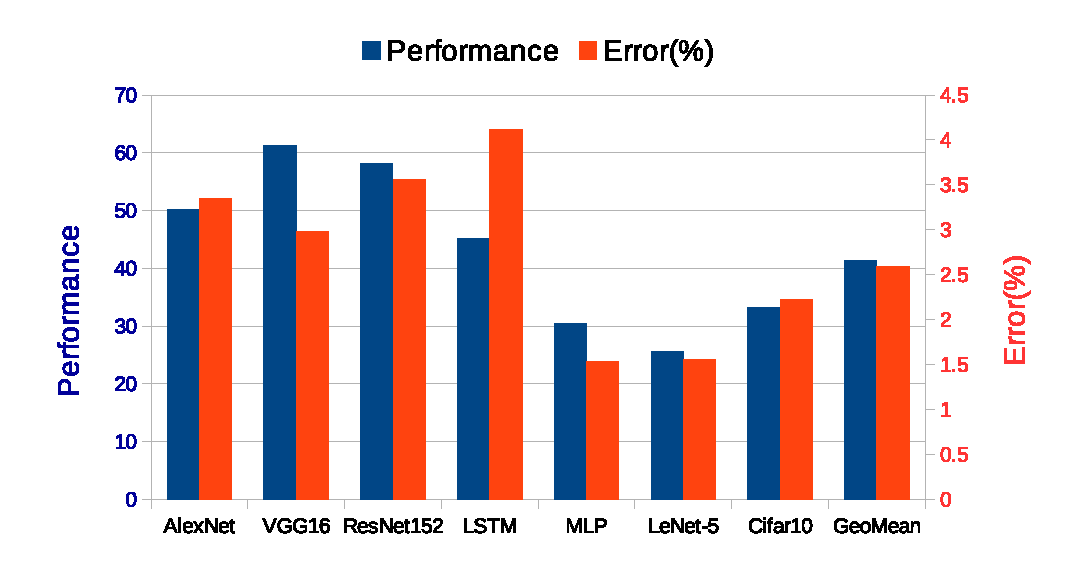
\includegraphics[width=1.0\columnwidth]{simulator.eps}
\caption{优化的模拟器与周期精确模拟器的对比}
\label{fig:simulator1}
\end{figure}



